%in_memory_file_system

\begin{figure}[t!]
\begin{center}
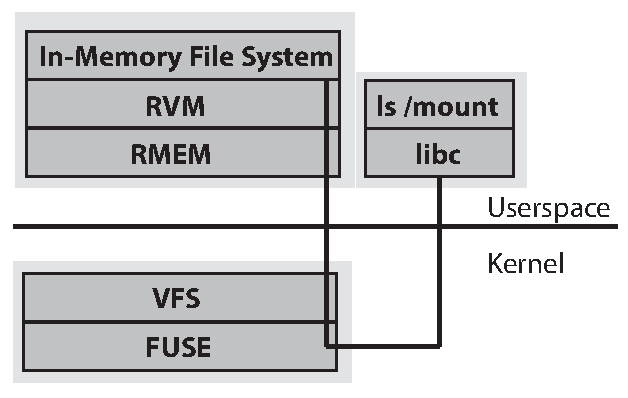
\includegraphics[scale=0.60]{graphs/inmem_fs_design.pdf}
\end{center}
\caption{In-memory file system design when using the RVM framework and FUSE library.}
\label{fig:inmem_fs_design}
\end{figure}

To demonstrate the flexibility and applicability of our framework we have applied our framework to RvmFS, a VFS compliant in-memory file system (see Figure~\ref{fig:inmem_fs_design}). 
RvmFS uses main memory as the only storage medium to provide very fast writes and reads. 
To be able to use our framework we have developed the file system using FUSE, a kernel module that allows the creation of user-space file systems.
RvmFS performs a commit of the file system in different situations: 1) an inode is created, 2) when a file is closed and 3) when a {\emph sync} operation is performed.

To evaluate the performance of the system we ran a subset of the benchmarks in the Filebench~\cite{filebench} benchmark suite. 
We compare the performance of the benchmark when running it against an ext4 file system backed by an SSD drive and when running on RvmFS backed by a remote server.
Table~\ref{tab:description} describes each specific benchmark that we ran and table~\ref{tab:results} shows the performance obtained.
We show the average latency of each operation in each benchmark.

\begin{table}[h]
\centering
\caption{Description of Macro Benchmark Tests. The file size of the randomread benchmark was reduced to simplify evaluation.}
\label{tab:description}
\resizebox{\columnwidth}{!}{%
    \begin{tabular}{ | l | c |} 
    \hline
    Benchmark name & Description \\
    \hline
    \hline
    file\_micro\_create  & \pbox{20cm}{Create an empty file and issue 1024 appends of 1MB each} \\
    \hline
    ramdomread  & \pbox{20cm}{Random reads (8K) from a file with size 1Mb} \\
    \hline
    openfiles  &  \pbox{20cm}{Creates a fileset with 500 empty files, \\then proceeds to open each one.} \\
    \hline
    \end{tabular}
}
\end{table}

\begin{table}[h]
\centering
\caption{Macro Benchmark Results}
\label{tab:results}
\resizebox{\columnwidth}{!}{%
\begin{tabular}{ | l | c | c |} 
    \hline
    \pbox{20cm}{Benchmark\\ name} & \pbox{20cm}{Latency per Op. (SSD)} & \pbox{20cm}{Latency per Op. (RvmFS)} \\
    \hline
    \hline
    file\_micro\_create  & 0.0004 sec & 21 sec\\
    \hline
    randomread  & 25us & 25us \\
    \hline
    openfiles  & 0 & 0 \\
    \hline
    \end{tabular}
}
\end{table}

\paragraph{Discussion}

As shown in Table~\ref{tab:results}, RvmFS is considerably slower for some specific benchmarks while obtaining similar performance in others.
The poor performance of the file system stems from different reasons.
First, some of the file system operations are not optimized for performance. For instance, when extending a file length, RvmFS allocates a new region of memory and copies all the file contents
to the new region. Not only copying all the data is slow, this also means that the next commit operation will backup the whole file contents even if only a small part of the file changed.
Secondly, RvmFS currently does not support multi-threaded access, common in modern file systems such as ext4.
Thirdly, RvmFS is ultimately limited by the performance of RVM. Due to the high overheads involved when backing up large contiguous regions of memory in RVM, RvmFS suffers.
Finally, RvmFS is not built with locality of storage in mind. This means that simple operations can touch many files.

Next we comment on the performance of each benchmark.

\paragraph{\bf file\_micro\_create}
The performance of RvmFS is far from the performance of ext4. This has to do with the inefficiency of RvmFS when extending the length of a file, as previously described.
\paragraph{\bf randomread} 
In this benchmark RvmFS has similar performance to the ext4 file system. Because the file being used to benchmark the read operations is small it can fit in memory. This favours ext4, which would have to perform disk reads if the file was bigger.
We will have to address the issue in the future.
\paragraph{\bf openfiles} 


% random read with ramfs
%26236: 61.739: Per-Operation Breakdown
%rand-read1           2440621ops    40675ops/s 317.8mb/s      0.0ms/op       12us/op-cpu [0ms - 0ms]
%26236: 61.739: IO Summary: 2440621 ops, 40674.879 ops/s, (40675/0 r/w), 317.8mb/s,     25us cpu/op,   0.0ms latency

% Random read with ssd
%26602: 61.006: Per-Operation Breakdown
%rand-read1           2435691ops    40592ops/s 317.1mb/s      0.0ms/op       12us/op-cpu [0ms - 0ms]
%26602: 61.006: IO Summary: 2435691 ops, 40592.390 ops/s, (40592/0 r/w), 317.1mb/s,     25us cpu/op,   0.0ms latency

% openfiles with ssd
%28390: 62.200: Per-Operation Breakdown
%close1               1095781ops    18262ops/s   0.0mb/s      0.0ms/op      590us/op-cpu [0ms - 0ms]
%open1                1095788ops    18262ops/s   0.0mb/s      0.0ms/op      587us/op-cpu [0ms - 0ms]
%28390: 62.200: IO Summary: 2191569 ops, 36524.045 ops/s, (0/0 r/w),   0.0mb/s,      0us cpu/op,   0.0ms latency


